%PART_1_CHAP_6
\myChapter[nteraction Homme Machine]{I}{nteraction homme machine}
\begin{resumChap}
Dans ce 6\ieme et dernier chapitre de cette partie, nous aborderons certains éléments caractéristiques de l'interaction homme-machine. \par%
Tout d'abord nous présenterons le concept de double-tâche rarement évitable dans ce contexte; la définition et le rôle des affordances; et, les effets qui peuvent être induits par le formalisme de la consigne donnée.\par%
Nous verrons également des notions d'utilisabilité indispensables à la conception d'interfaces permettant l'interaction.\par%
Et enfin, nous verrons comment ces technologies une fois développées (et utilisables) peuvent être acceptées par les utilisateurs dans leurs pratiques quotidiennes.\end{resumChap}{}
%WAIT a Review ok
\section{Ergonomie des interfaces}
    \subsection{La double tâche}\label{sec:double-tache}
        Dans le monde numérique actuel il est fréquent de devoir partager son attention sur plusieurs points de l'espace. Mais l'utilisateur doit pouvoir conserver suffisamment de ressources cognitives pour planifier son action. Ainsi, se trouvant régulièrement en double tâche (voir en multi-tâches) l'utilisateur doit être capable de gérer ses ressources pour répondre et interagir, de la manière la plus efficiente possible, avec son environnement.\par%
        Nombreuses sont les personnes à avoir l’impression d’être performantes dans ces situations, par exemple, être capable de conduire et de tenir une conversation simultanément; or, cette impression est biaisée car la conduite est une action automatisée, elle est donc inconsciente et elle ne mobilise que peu de ressources attentionnelles. c'est un fait, dès que nous nous engageons dans deux activités conscientes en même temps, l’une ou l’autre des activités en souffrira car le cerveau humain a beaucoup de mal à distribuer son attention sur plusieurs tâches simultanément \eg exemple de la cécité attentionnelle (Inattentional blindness): le gorille invisible~\citeB{drew2013invisible}. En fait, l’impression d’être multitâche n’est rien d’autre que le fait de passer d’une tâche à l’autre très vite et donc, le plus souvent, au détriment de la qualité des deux~\citeB{pashler1994dual}.\par%
        Dans notre cadre, l'utilisateur, l'élève, doit être capable d'organiser son attention pour d'abord comprendre les consignes et établir un plan pour atteindre l'objectif. Puis il doit partager son attention sur, au moins, 2 points de l'espace: la fenêtre permettant l'exécution du code (l'interface) et l'exécution du comportement dans le simulateur \etou sur un robot réel. Enfin, il doit pouvoir comparer et analyser les deux phénomènes issus de cette démarche: l'asymétrie entre le comportement voulu et le comportement produit, et l'asymétrie entre son exécution sur un modèle simulé et sur un modèle réel. Et toutes ces étapes: conception du code, rédaction, exécution, analyse du comportement, comparaison; doivent être itérées de nombreuses fois pour obtenir un résultat satisfaisant.
        Afin de réduire la charge cognitive immédiate pour les utilisateurs novices de la plateforme, une première idée est de segmenter les séquences (\ie les décomposer en plusieurs objectifs distincts). 
        %Une seconde idée serait de concevoir des itinéraires d'acquisition de compétences se présentant sous la forme d'un poly-arbre à l'instar du développement de la compétence motrice bipède chez les enfants. En effet l'acquisition de cette compétence peut  transiter, ou non, par différentes phases plus ou moins atypiques (e.g marche quadrupède, déplacement sur les fesses, utilisation de supports, \etc).
        %Ces trajectoires développementales variées sont fréquemment observées dans l'environnement naturel, il semble donc logique d'imaginer des supports pédagogiques possédant la même souplesse pour apprendre des schèmes logiques que pour l'apprentissage naturel des schèmes moteurs.
    \subsection{Les affordances}\label{sec:affordance}
        \paragraph{Selon Gibson}
            C'est en 1977 dans \textit{The Theory of Affordances} par James~J. Gibson ~\citeB{gibson1977theory} qu'apparaît le terme affordance. Deux ans plus tard, il le précise dans l'Approche écologique de la perception visuelle~\citeB{gibson1979theory}. Pour lui, l'affordance est l'ensemble de toutes les possibilités d'action d'un environnement~\citeB{greeno1994gibson}. Elle sont objectives, cependant elles doivent toujours être mises en relation avec l'acteur qui peut les utiliser \eg pour un nourrisson, un escalier n'a pas l'affordance d'être escaladé. L'affordance est suggérée par l'objet lui-même: elle est une partie constitutive de ce dernier; Elle ne naît donc pas des besoins de l'utilisateur ni de son action de perception. Toutefois, les affordances ne sont pas, pour Gibson, des propriétés à part entière de l'objet mais plutôt des combinaisons invariantes de variables qui dépendraient du contexte de l'action.
        \paragraph{Selon Norman}
            Pour Donald Norman \tiret{qui réutilise le terme dans \textit{The Design of Everyday Things} en 1988~\citeB{norman1988psychology}}, l'affordance, dans le cadre de l'\sht{IHM}, désigne les potentialités d'action perceptibles par l'utilisateur d'un programme. En 2013, il revient sur cette notion et insiste sur la différence entre affordance (l'interaction potentielle) et signifier (le moyen de communiquer cette potentialité)~\citeB{norman2013design}.
        \paragraph{Plus généralement}
            Le terme d'affordance est emprunté à l’anglais et peut se traduire par \gui{potentialité}. Il dérive du verbe \cro{\textit{to afford}} qui a un double sens: \gui{être en mesure de faire quelque chose} et \gui{offrir}.
            Le terme se retrouve dans différents domaines, notamment la psychologie cognitive, la psychologie de la perception, la psychologie ergonomique, le design, l'\bg{IHM} et l'\bg{IA}. Deux grandes voies de définition se sont développées:
            \begin{enumerate}\myItemStyle
                \item C'est de la psychologie que provient la définition originale de l'affordance: elle désigne \gui{toutes les possibilités d'action sur un objet}. Puis, cette définition s'est restreinte aux seules possibilités dont l'acteur est conscient.
                \item En ergonomie, le terme se restreint un peu plus pour se référer uniquement à la \gui{capacité d’un objet à suggérer sa propre utilisation}, \ie sans qu'il ne soit nécessaire de lire un mode d'emploi. On parle alors d'utilisation intuitive d'un objet ou de son caractère intuitif.
            \end{enumerate}{}
        \paragraph{Selon Gaver}
            Il y aurait 2 types d'affordances: \Li le type séquentiel et \ii le type spatial qui sont associés à 3 qualités perceptuelles: perceptible, dissimulée, ou trompeuse~\citeB{gaver1991technology}.
            \subparagraph{Affordances séquentielles}
                La notion d'affordance séquentielle (sequential affordance) réfère aux situations où l'action sur une 1\iere affordance perceptible donne des informations sur une 2\nde affordance dissimulée devenant alors perceptible. Il y a donc ici une notion de temporalité.
            \subparagraph{Affordances spatiales}
                Les affordances spatiales se réfèrent quant à elles, à leur groupement dans l'espace. Par exemple une porte suggère qu'elle peut s'ouvrir par sa séparation du mur, mais n'indique pas forcément si elle doit être coulissée, poussée ou tirée; le type de poignée de la porte pourra lever ce doute si elle semble, par exemple, pouvoir être poussée plutôt que tirée. C'est donc grâce au groupement spatial de la poignée par rapport à la porte que l'on perçoit l'affordance et donc quelle action il faut effectuer.
            \subparagraph{Affordance et perception}
                William Gaver introduit le rapport entre l'affordance et la perception de celle-ci en 3 catégories:
                \begin{figure}[!h]
                \begin{minipage}{0.45\linewidth}
                    \centering
                    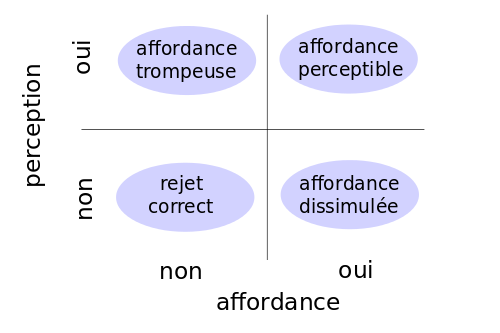
\includegraphics[width=\linewidth]{Figures/Gaver-Cat_affordances.png}
                    \caption{Catégorisation affordances - perception, Gaver~\citeB{gaver1991technology}}
                    \label{fig:affordance}
                \end{minipage}
                \begin{minipage}{0.495\linewidth}
                \myDefautStyle
                    \begin{itemize}\myItemStyle
                        \item Affordance perceptible: Un objet permet une action et la suggère. Par exemple, la forme et position d'une poignée de porte suggère d'utiliser sa main et de tourner afin d'ouvrir la porte, tandis que la forme et la position d'une pédale de voiture suggère d'appuyer avec le pied.
                    \end{itemize}{}\par%
                \end{minipage}
                \myDefautStyle
                \begin{itemize}\myItemStyle
                    \item Affordance dissimulée: Un objet permet une action mais ne la suggère pas directement. Utiliser un coin de table pour décapsuler une bouteille est une affordance dissimulée alors que la forme d'un décapsuleur rend son affordance perceptible. Ainsi, se rendre compte et utiliser une affordance dissimulée peut par exemple référer à une utilisation détournée de l'objet ou à une fonctionnalité que le designer de l'objet n'a pas su, ou n'avait pas l'intention, de rendre explicite.
                    \item Affordance trompeuse (false affordance): Un objet suggère une action qu'il ne permet pas. Un bouton placebo en est un exemple
                \end{itemize}{}
                \end{figure}{}
    \subsection{rôle de la consigne}
        \begin{figure}[!h]
              \centering
              \label{fig:Candle_Problem}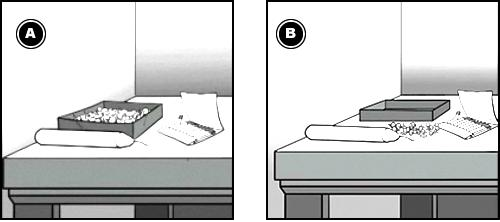
\includegraphics[width=\linewidth]{Figures/Dunckers-candle_problem.png}
              \caption{Candle Problem~\citeB{duncker1945problem}}
        \end{figure}\par%
        Une fois le rôle de chaque acteur et l'importance du support cadrés, il faut construire le matériel pédagogique adéquat. Avoir conscience de certains principes psychologiques déjà établis est indispensable. Un exemple parmi d'autres est l'expérience de la bougie (Dunker, K.~\citeB{duncker1945problem}) où est mis en évidence la contrainte émise par la situation initiale sur l'efficacité à résoudre une tâche. Ici, la consigne est identique \gui{fixer la chandelle au mur sur un tableau de liège sans que la cire tombe sur la table située en dessous} mais, le matériel à disposition pour réaliser cette tâche n'est pas disposé de la même manière et ne fournit pas les mêmes affordances. Ceci a un impact direct sur la capacité à réussir la tâche.
        Cependant, dans l'élaboration d'objectifs complexes, il est difficile d'estimer l'ensemble des conséquences qu'aura tel ou tel type de consigne. Cependant des principes généraux d'ergonomie des interfaces permettent de limiter les fourvoiements.
        %Avoir conscience des répercutions de donner un objectif lors de la rédaction de séquences pédagogiques est indispensable. 
        %\AreF{déjà dit}{Dès 1945, Duncker[5] montrait dans son expérience de la bougie le rôle crucial de la consigne sur l'efficacité à résoudre une tâche. 
\section{Utilisabilité}\label{sec:utilisabilite}
    \subsection{Définition}
        Plusieurs concepts et normes de conception ont déjà été théorisés. Parmi ces concepts les plus connus sont certainement les 7 critères de Bastien~et~Scapin~\citeB{scapin1997ergonomic} ou les dix heuristiques de Nielsen~\citeB{nielsen1994usability}. Ces références datent des années 1990 pourtant elles restent d'actualité et sont régulièrement citées lors de la rédaction de normes, telles les normes ISO (\textit{ISO 9241-11}) et Afnor (\textit{Norme Z67-133-1}).
        La norme ISO, la plus communément citée, définie l'utilisabilité ainsi:
        \citeAtion{ISO}
        \paragraph{Efficacité} 
            L'efficacité est la capacité, d'une personne, d'un groupe ou d'un système, à parvenir à ses fins, à ses objectifs (ou à ceux qu'on lui a fixé). Être efficace revient à produire à l'échéance prévue les résultats escomptés et réaliser des objectifs fixés, objectifs qui peuvent être définis en terme de quantité, mais aussi de qualité, de rapidité, de coût, de rentabilité, \etc. 
        \paragraph{Efficience}
            L'efficience est un composant important de la mesure de la performance. C'est l'optimisation de la consommation des ressources utilisées (entrant; matière ou énergie) dans la production d'un résultat (sortant). De ce fait, elle peut se mesurer à partir de rapports entre les résultats obtenus et les ressources utilisées.
        \paragraph{Gibert, Modèle de la performance}
        \strut%\newline\strut
        \begin{figure}[!h]
                \begin{minipage}{0.435\linewidth}
                \centering
                    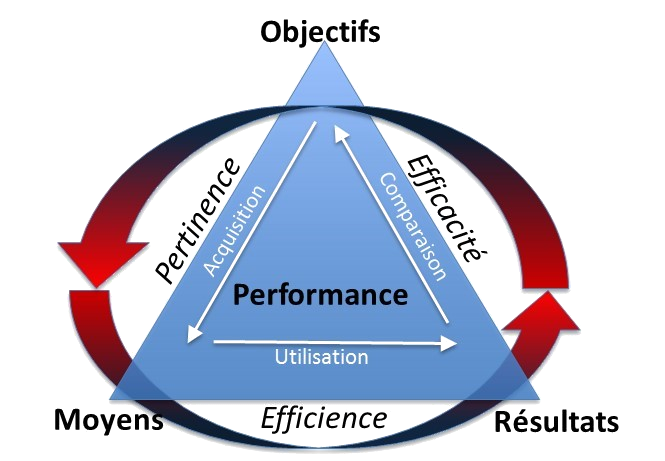
\includegraphics[width=\linewidth]{Figures/Gibert-Modele_performance.png}
                    \caption{Triangle de la performance, Gibert~\citeB{gibert1980controle}}
                    \label{fig:perf_gibert}
                \end{minipage}
                \hfill
                \begin{minipage}{0.55\linewidth}
                \myDefautStyle
                    En conformité avec le modèle de Gilbert, il faut la distinguer de l'efficacité, qui vise à vérifier si les résultats obtenus sont en ligne avec les objectifs fixés, et de la pertinence, qui vise à procurer les moyens suffisants et adéquats pour atteindre les objectifs fixés.\par\vspace{1cm}
                \end{minipage}
        \end{figure}{}\par%
        \paragraph{Satisfaction}
            Usuellement, la satisfaction correspond au nom donné à l’état d’âme (ou du corps) qui accompagne l’accomplissement d'un désir ou l'assouvissement d'un besoin (l'achèvement d’un besoin). De manière plus restreinte, la satisfaction utilisateur, ou satisfaction client ou encore satisfaction consommateur, est un concept issu des standards de gestion de la qualité (ISO 9000~\citeUrl{ISOstatisfaction}) où la satisfaction est la finalité de la mise en place de processus.
            %Une entreprise apporte au client un produit ou un service. 
            La satisfaction est donc ici une perception des qualités intrinsèques du produit ou service fourni par rapport aux besoins exprimés par le consommateur.
            %Cette satisfaction est mesurée par les entreprises, par des indicateurs qualitatifs, pour améliorer sans cesse la satisfaction: la fidélité du client est le but de cette surveillance, voire le fait qu'il devienne ambassadeur du produit ou de la marque. Une entreprise sans client n'a plus de raison d'être. Les retours des clients sur leurs insatisfactions sont de plus, l'opportunité de travailler à les résoudre et ainsi améliorer son indicateur de satisfaction.
            %Plusieurs entreprises indiquent ainsi qu'un client satisfait est un facteur d'accroissement de la profitabilité, une relation entre la satisfaction et les niveaux de trésorerie étant constatée. Le président d'Amazon France, Romain Voog, indique ainsi qu'\gui{un acheteur satisfait représente, au final, une dizaine de clients recrutés.}. Un autre exemple concerne la SNCF qui mesure continuellement la satisfaction de ses clients, et notamment la ponctualité de ses trains. La directrice générale de SNCF Voyageurs indique que \gui{la mission de la SNCF est de répondre aux besoins de chacun de nos voyageurs et leur satisfaction est la priorité absolue de chaque cheminot.}. 
    \subsection{Les critères de Bastien et Scapin}
        En 1997, Bastien et Scapin présentent dans \textit{Ergonomic criteria for evaluating the ergonomic quality of interactive systems}~\cite{scapin1997ergonomic} une série de critères permettant de mieux catégoriser les défauts d’ergonomie, de juger de leur importance et de trouver des solutions pour les résoudre. Ces critères doivent être gardés à l’esprit lors de la conception afin de prendre en compte l’ensemble des facteurs favorisant l’ergonomie d’une application, d’un service ou d’un site web.
        \paragraph{1. Guidage}
            Le guidage correspond aux éléments présents pour conseiller, orienter, informer, et conduire l’utilisateur lors de ses interactions avec le système (messages, alarmes, labels, \etc). Quatre sous-critères participent au Guidage: Incitation, Groupement/Distinction entre Items, Feedback Immédiat et Lisibilité.
            \subparagraph{Incitation}
                Ce critère correspond aux informations permettant aux utilisateurs de savoir où ils en sont, d’identifier l’état et le contexte dans lequel ils se trouvent. Il englobe aussi tous les mécanismes permettant de faire connaître aux utilisateurs ses alternatives, lorsque plusieurs actions sont possibles. Plus généralement, il correspond à toutes les mises en œuvre pour amener les utilisateurs à effectuer des actions spécifiques dans un contexte donné.
            \subparagraph{Groupement et Distinction}
                Il s'agit ici de l’organisation visuelle des items présents dans le contexte. Ce critère prend en compte la topologie (la localisation) et certaines caractéristiques graphiques (le format) afin d’illustrer les relations entre les divers items affichés.%leur appartenance ou non- appartenance à une même classe, ou encore dans le but de montrer la distinction entre différentes classes d’items. 
                %Ce critère concerne aussi l’organisation des items à l’intérieur d’une même classe. Deux sous-critères participent au Groupement/Distinction entre Items: Groupement/Distinction par la Localisation et Groupement/Distinction par le Format.
            \subparagraph{Feedback Immédiat}
                Suite à une action de l'utilisateur, allant du simple appui sur une touche à l’entrée d’une séquence complexe de commandes, la réponse donnée par le système: le feedback, doit être aussi immédiate que possible et fournir à l’utilisateur le renseignant sur l’action accomplie et sur son résultat.
                %concerne les réponses de l’ordinateur consécutives aux actions des utilisateurs, lesquelles peuvent être le simple appui sur une touche ou l’entrée d’une séquence de commandes. Dans tous les cas, l’ordinateur doit répondre, dans les plus brefs délais, avec un délai de réponse approprié et homogène selon les types de transactions. Dans tous les cas, 
            \subparagraph{Lisibilité}
                Par convention, le critère de lisibilité ne concerne ni le feedback ni les messages d’erreurs. Il renvoie aux caractéristiques lexicales de présentation des informations sur l’écran pouvant entraver ou faciliter la lecture de ces informations (luminance, contraste, fond, dimension, espacement, \etc). 
        \paragraph{2. Charge de Travail}
            La charge de travail correspond à l’ensemble des éléments présents dans l’interface qui ont pour objectif de réduire la charge perceptive (ou mnésique) des utilisateurs. Deux sous-critères y participent: la brièveté (qui inclut les critères de \cro{concision} et d'\cro{actions minimales}), et la densité informationnelle.
            \subparagraph{Brièveté}
                Il s’agit ici de limiter \tiret{autant que possible} le travail de lecture, d’entrée et les étapes par lesquelles doivent passer les utilisateurs (\ie les suites d’actions nécessaires à l’atteinte d’un but, à l’accomplissement d’une tâche).
            \subparagraph{Densité Informationnelle}
                La charge de travail, en terme de densité informationnelle, correspond à la quantité d'information perceptive et mnésique stockée par l'utilisateur, et non, à la densité des items qui lui sont présentés.
        \paragraph{3. Contrôle Explicite}
            Le contrôle explicite concerne à la fois la prise en compte par le système des actions explicites des utilisateurs et le contrôle qu’ont les utilisateurs sur le traitement de leurs actions. Deux sous-critères y participent:
            \subparagraph{Actions Explicites}
                Les relations pouvant exister entre le fonctionnement de l’application et les actions des utilisateurs doivent être explicites, \cad que le système doit exécuter (en premier plan) uniquement les opérations demandées par l’utilisateur et pas d’autres et ce, au moment où il les demande.
            \subparagraph{Contrôle Utilisateur}
                L’utilisateur doit toujours avoir la main, pouvoir contrôler le déroulement (\eg interrompre, reprendre une séquence d'exécution) des traitements informatiques en cours.
        \paragraph{4. Adaptabilité}
            L'adaptabilité d’un système correspond à sa capacité à réagir selon le contexte, et selon les besoins et préférences des utilisateurs. Deux sous-critères y participent:
            \subparagraph{Flexibilité}
                Le critère de flexibilité correspond au nombre de façons différentes mises à la disposition des utilisateurs pour atteindre un objectif donné dans le but de lui permettre de personnaliser l’interface pour s'adapter à ses stratégies ou habitudes de travail ou encore aux exigences de la tâche.
            \subparagraph{Prise en compte de l’expérience de l’utilisateur}
                concerne les moyens mis en œuvre pour respecter le niveau d’expérience de l’utilisateur.
        \paragraph{5. Gestion des Erreurs}
            Ce critère concerne tous les moyens permettant d’une part d’éviter \tiret{ou de réduire} les erreurs, et d’autre part de les corriger lorsqu’elles surviennent. Les erreurs sont ici considérées comme des saisies de données incorrectes (\eg des saisies dans des formats inadéquats, des commandes avec une syntaxe incorrecte, \etc). Trois sous-critères y participent:
            \subparagraph{Protection contre les Erreurs}
                C'est un moyen mis en place pour détecter et prévenir les erreurs d’entrées de données ou de commandes ou les actions aux conséquences néfastes.
            \subparagraph{Qualité des Messages d’Erreur}
                En d'autres termes la pertinence, la facilité de lecture et l’exactitude de l’information donnée aux utilisateurs sur la nature des erreurs commises (syntaxe, format, \etc) et sur les actions à entreprendre pour les corriger.
            \subparagraph{Correction des Erreurs}
                Ce sous-critère fait référence aux moyens mis à la disposition des utilisateurs pour leur permettre de corriger leurs erreurs.
        \paragraph{6. Homogénéité et Cohérence}
            L'homogénéité et la cohérence renvoient à la façon avec laquelle les choix de conception de l’interface sont conservés pour des contextes identiques, et différents pour des contextes différents.
        \paragraph{7. Signifiance}
            La signifiance des \cro{codes et dénominations} fait référence à l’adéquation entre l’objet ou l’information affichée ou entrée, et son référent. Des codes et dénominations dits signifiants ont une relation sémantique forte avec leur référent.
        \paragraph{8. Compatibilité}
            Ce dernier critère se réfère à l’accord pouvant exister entre les caractéristiques des utilisateurs (mémoire, perceptions, habitudes, compétences, âge, attentes, \etc) et des tâches, d’une part, et l’organisation des sorties, des entrées et du dialogue d’une application donnée, d’autre part. De plus, la compatibilité concerne également le degré de similitude entre divers environnements ou applications. 
    \subsection{Les 10 heuristiques de Nielsen}
        Avant Bastien et Scapin, Nielsen, en 1994 dans \textit{Usability Engineering}~\cite{nielsen1994usability} proposaient déjà une série de critères: 10 heuristiques, permettant de mieux concevoir les systèmes interactifs.
        \paragraph{1. Visibilité de l’état du système}
            Tenir informé l’utilisateur de ce qui se passe: donner un feedback approprié dans un délai raisonnable.
        \paragraph{2. Correspondance du système avec le monde réel}
            L'interface doit \gui{parler} le langage de l’utilisateur, avec des mots, des phrases et des concepts qui lui sont familiers (conventions du monde réel)
        \paragraph{3. Liberté, contrôle de l’utilisateur}
            Comme l'utilisateur peut choisir, par erreur, certaines fonctions du système, celui-ci doit lui offrir des fonctions d’annulation à tout moment.
        \paragraph{4. Cohérence et standards}
            Le système doit être conforme au mode de représentation de l’utilisateur et respecter les standards d’utilisation.
        \paragraph{5. Prévention des erreurs}
            Le design doit permettre de prévenir (anticiper) les problèmes que pourrait rencontrer l’utilisateur.
        \paragraph{6. Reconnaître plutôt que se souvenir}
            Les instructions pour utiliser le système doivent être immédiatement visibles ou facilement accessibles.
        \paragraph{7. Flexibilité et efficacité de l’utilisation}
            Les raccourcis \tiret{ignorés par des utilisateurs novices} permettent souvent d’accélérer les interactions pour les utilisateurs expérimentés. Ainsi, donner la possibilité d’automatiser les actions récurrentes permet d'améliorer l'efficience des utilisateurs expérimentés. 
        \paragraph{8. Esthétique et design minimaliste}
            Les informations qui ne sont pas pertinentes ou qui ne sont que rarement nécessaires doivent être limitées ou contextuelles car elles diminuent la visibilité des informations pertinentes.
        \paragraph{9. Faciliter l’identification et la gestion des erreurs}
            Les messages d’erreur doivent être formulés en langage clair, indiquer précisément le problème et suggérer une solution pour le résoudre.
        \paragraph{10 Aide et documentation}
            Bien qu’il soit préférable que le système puisse être utilisé sans le recours à une documentation, il peut être nécessaire d’en fournir à l’utilisateur avec une facilité d’accès.
    \subsection{D'autres critères}
        Nous voyons que les critères énoncés par Bastien et Scapin d'un côté et Nielsen de l'autre sont très similaires, ce qui montre une certaine cohérence dans les éléments significatifs à prendre en considération. D'autres \textit{guideline} existent comme les \textit{check-lists} d'évaluation ergonomique et de conception d'un site Web proposé par Nogier~\cite{nogier2002ergonomie} ou la check-list logicielle basée sur la Norme ISO 9241 de Ribeiro~\citeUrl{ISOcritere}.
%TODO
\begin{comment}
% suprimé pour dépot le 24/10, à finir pour envoie au rapporteur le 28/10
\section{Appropriation}
    \nocite{proulx2002trajectoires}\myL{3}%TODO
    A. [L'idée dominante est celle d'adaptation] Action d'adapter quelque chose à un usage déterminé.
    B. [L'idée dominante est celle de propriété] 1. Action de s'approprier une chose, d'en faire sa propriété; 2. Acte de l'esprit qui s'approprie, qui fait siennes les connaissances qu'il acquiert. Synon. assimilation.
    \url{https://www.cnrtl.fr/definition/appropriation}
\end{comment}
\section{Acceptabilité}\label{sec:acceptable}
    Mais l'utilisabilité d'un système ne crée pas nécessairement son acceptation. L'acceptabilité d'une technologie dépend de beaucoup de facteurs. En premier lieu elle dépend de son utilité perçue, caractère extrêmement subjectif qui prend naissance avant même la première interaction entre le système et l'utilisateur. 
    Cette notion d'utilité perçue est primordiale, et pour satisfaire celle-ci, la technologie doit se baser sur les besoins de la personne mais surtout sur ses envies et ses a priori. Tous ces paramètres sont extrêmement variables d'une population à l'autre car il varie en fonction des us et coutumes, des normes sociales, qui varient en fonction des CSP, des âges, \etc. 
    \subsection{Le modèle TAM}
        Cependant l'utilité perçue (notée U) n'est qu'un des facteurs rendant compte de l'acceptabilité d'une technologie. Ainsi déjà en 1989 Davis présentait le modèle TAM (Technologie Acceptance Model)~\citeB{davis1989user,lee2003technology} mettant en liaison plusieurs concepts permettant de mieux définir l'utilisation réelle d'une technologie faite par son utilisateur et donc l'acceptation de celle-ci. Voici ses concepts: utilité perçue (notée U) - simplicité d'utilisation perçue (E) - attitude envers l'utilisation du système (A) - intention d'utilisation (BI). 
        \begin{figure}[!h]
              \centering
              \label{fig:TamModel}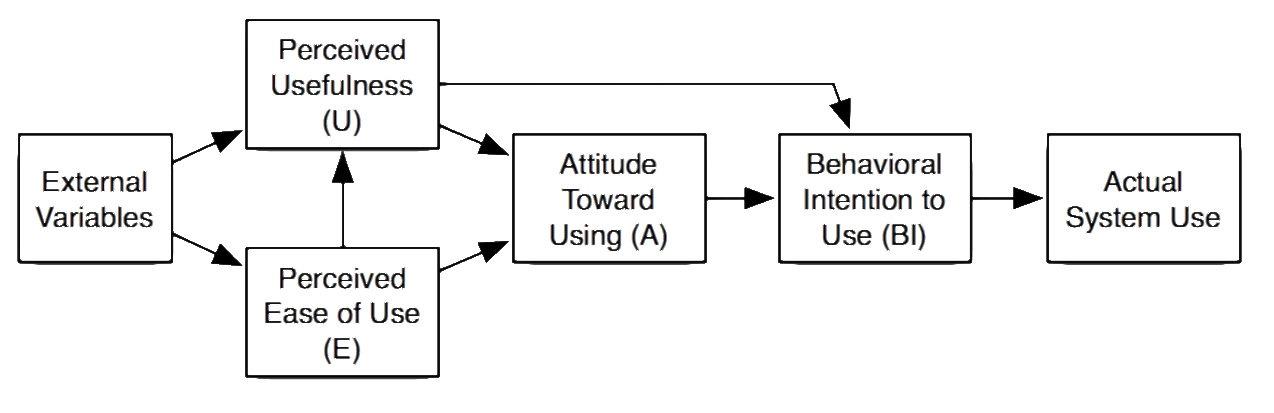
\includegraphics[width=\linewidth]{Figures/Davis-TAM_Model.png}
              \caption{Modèle TAM~\citeB{davis1989user}}
        \end{figure}\par%
        On peut voir sur ce schéma qu'il y a une vraie interaction non-linéaire entre ces concepts, marquant une fois de plus la complexité de vouloir répondre de manière généralisée à des concepts liés inexorablement au caractère subjectif des individus. 
    \subsection{Le modèle UTAM}    
        D'autres ont cherché des représentations plus complexes comme Venkatesh en 2012 qui présente le modèle:
        \begin{figure}[!h]
              \centering
              \label{fig:UTamModel}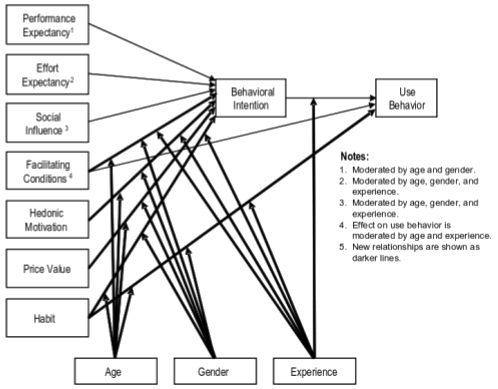
\includegraphics[width=\linewidth]{Figures/venkatesh-UTAM_Model.png}
              \caption{Modèle UTAM~\citeB{venkatesh2012consumer}}
        \end{figure}\par%
        On voit ici que trois concepts agissent directement sur le comportement d'utilisation, comportement qui permet alors de prédire si une technologie sera acceptée ou non. Comme dans le modèle TAM on retrouve le concept d'intention d'utilisation (behavioral intention) mais en parallèle on trouve les conditions d'utilisation (contexte, environnement, \etc) et les habitudes qu'ont déjà les utilisateurs et les affordances associées. 
        Une autre différence notable entre les deux modèles est la présence des modulateurs âge, sexe et expérience. Ceux-ci ont une influence sur la majeure partie des branches sans pour autant être directement assimilés à des facteurs directs pouvant agir sur le résultat final: ils doivent s'exprimer à travers d'autres concepts.
        Une limite à ces modèles est qu'ils ne prennent pas en compte la notion de rétroaction, où le comportement d'utilisation actuel agit sur les variables d'entrée. Comme par exemple avec de nouvelles habitudes ou avec le changement d'estimations des performances/efforts à accomplir via le système pour réaliser une tâche.